\documentclass[10pt]{article}
\usepackage[utf8]{inputenc}
\usepackage[T1]{fontenc}
\usepackage{amsmath}
\usepackage{amsfonts}
\usepackage{amssymb}
\usepackage[version=4]{mhchem}
\usepackage{stmaryrd}
\usepackage{graphicx}
\usepackage[export]{adjustbox}
\graphicspath{ {./images/} }

\title{Übungsblatt 5 }


\author{Prof. Dr.-Ing. Lars Linsen\\
Adrian Derstroff\\
Marina Evers\\
Karim Huesmann}
\date{}


\begin{document}
\maketitle
Informatik 1, WiSe $2022 / 23$



\begin{abstract}
Abgabefrist: Montag, den 21.11.22, bis 12:00 Uhr (nicht 24:00 Uhr). Wenn es nicht explizit von der Aufgabe gefordert wird, benutzen Sie für Ihre Lösungen im 
 Programmcode nur Klassen und Methoden, die in der Vorlesung vorgestellt wurden. Geben Sie alle theoretischen Aufgaben jeweils als PDF ab. Achten Sie bei der Abgabe von Fotos oder Scans bitte auf Lesbarkeit. Haskell-Code soll als .hs-Datei und als PDF abgegeben werden.
\end{abstract}

Aufgabe T5.1: Code verstehen

$(1+1=2$ Punkte $)$

Sie finden online einen fertigen Programmcode, der wohl etwas hastig geschrieben wurde. Die sehr ineffizient gestaltete Funktion wurde wie folgt implementiert:

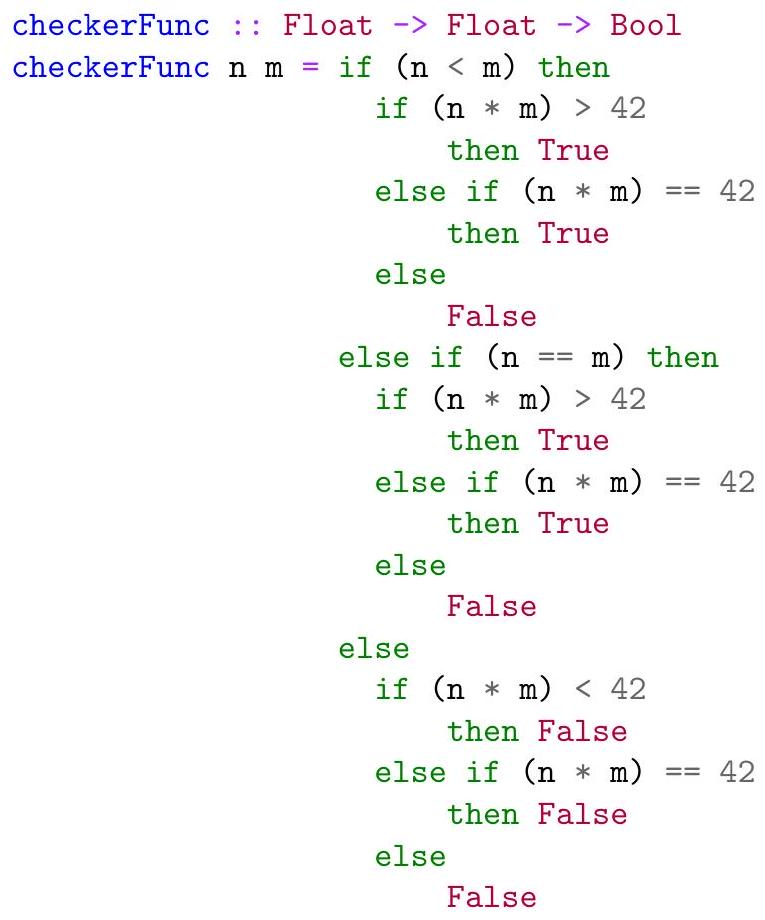
\includegraphics[max width=\textwidth]{2022_11_15_0a5a2eee0aef383b0ce9g-1}

(a) Fassen Sie zusammen, welche Eigenschaften von $n$ und $m$ erfüllt sein müssen, damit die Funktion True zurückgibt.

(b) Die Funktion lässt sich in einem einzigen booleschen Ausdruck darstellen. Geben Sie die entsprechende Funktion als Haskellcode (schriftlich) an.

Aufgabe T5.2: Abgeleitete Klassen

(2 Punkte)

In der Vorlesung haben sie Standard-Typklassen wie Ord, Enum oder Num kennengelernt. Im folgenden Programmcode wird ein neuer Datentyp Season definiert:

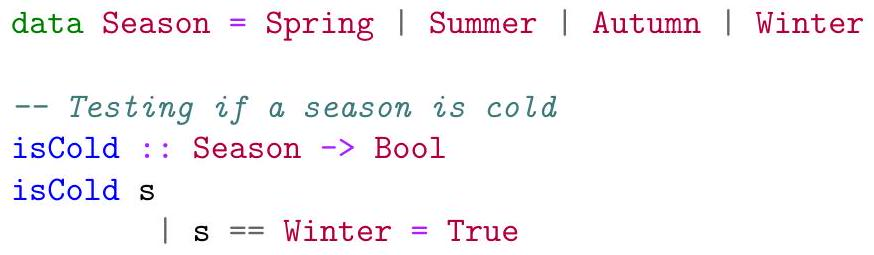
\includegraphics[max width=\textwidth]{2022_11_15_0a5a2eee0aef383b0ce9g-1(1)}

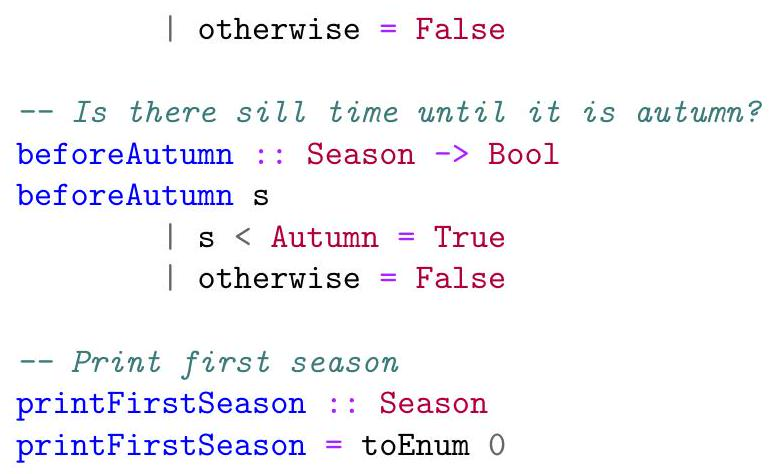
\includegraphics[max width=\textwidth]{2022_11_15_0a5a2eee0aef383b0ce9g-2}

Ausgehend von den gegebenen Funktionen, überprüfen Sie, ob für die neue Klasse alle notwendigen Standard-Typklassen in Form einer abgeleiteten Instanzdeklaration angegeben worden sind. Falls nicht, fügen Sie diese noch hinzu und begründen Sie Ihre Antwort.

Hinweis: Verwenden Sie nur die in aus der Vorlesung bekannten Standard-Typklassen.

Aufgabe P5.3: Klassen $(1+2+5=8$ Punkte $)$

In der Vorlesung wurden die Datentypen Point und Vector umgesetzt. Nun soll eine Klasse Polygon implementiert werden. Dabei ist ein Polygon eine Menge von Punkten. Die Klasse Polygon definiert die Funktionen:

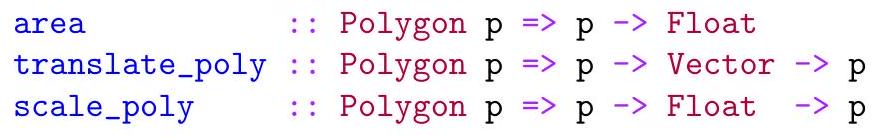
\includegraphics[max width=\textwidth]{2022_11_15_0a5a2eee0aef383b0ce9g-2(1)}

Dabei nimmt die Funktion area ein Polygon entgegen und gibt die Fläche des Polygons zurück. Die Funktion translate verschiebt jeden Punkt eines Polygons. Die Verschiebung wird durch einen Vektor angegeben. Die Funktion gibt danach das verschobene Polygon zurück. Die Funktion scale multipliziert jeden Punkt eines Polygons mit einer Gleitkommazahl $s$ und gibt das skalierte Polygon zurück. Die Ergebnisse aller Funktionen sollen in der Konsole angezeigt werden können. Bearbeiten Sie nun folgende Aufgaben:

(a) Implementieren Sie die Datentypen Point und Vector, die Sie in der Vorlesung kennengelernt haben. Dabei sollen die beiden Datentypen keine alternative Schreibweise für Tupel sein, sondern als eigene Datentypen definiert werden. Implementieren Sie die Funktionen translate und scale mit folgender Signatur:

translate : : Point $\rightarrow$ Vector $\rightarrow$ Point

scale : : Point $\rightarrow$ Float $\rightarrow$ Point

Dabei verschiebt die Funktion translate einen Punkt um einen Vektor und die Funktion scale multipliziert einen Punkt komponentenweise mit einer Gleitkommazahl.

(b) Definieren Sie die Klasse Polygon und die Datentypen Triangle (allgemeines Dreieck) und Quad (allgemeines Viereck).

(c) Implementieren Sie die Datentypen Triangle und Quad als Instanzen von der Klasse Polygon und implementieren Sie dabei die von der Klasse Polygon definierten Funktionen.

Hinweis: Falls notwendig, recherchieren Sie die Formeln für die benötigten Flächenberechnungen.

Aufgabe P5.4: Aufzählung $(1+2+3=6$ Punkte $)$

Es soll eine Klasse Card für Spielkarten implementiert werden. Eine Spielkarte besteht aus einem Rank (Wert) \{Seven, Eight, Nine, Ten, Jack, Queen, King, Ace\} in aufsteigender Reihenfolge und einem Suit (Farbe) $\{$ Diamond, Heart, Spade, Club $\}$.

(a) Implementieren Sie die Datentypen Rank, Suit und Card.

(b) Implementieren Sie Card als eine Instanz der Klasse Ord. Dabei entscheidet der Wert (Rank) welche Karte größer ist, bei zwei Karten gleichen Wertes entscheidet die Farbe (Suit), welche Karte größer ist. Bei gleichem Wert und gleicher Farbe sind beide Karten gleich groß. (c) Implementieren Sie den Datentypen Hand, der aus drei Karten besteht. Implementieren Sie anschließend eine Funktion value :: Hand $\rightarrow$ Integer, welchen den Wert der Hand zurückgibt. Dabei seien folgende Handkombinationen definiert:

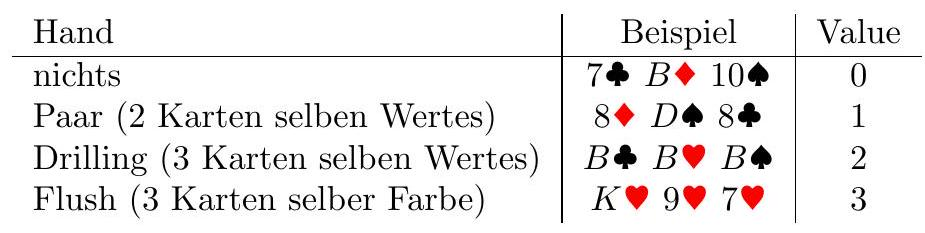
\includegraphics[max width=\textwidth]{2022_11_15_0a5a2eee0aef383b0ce9g-3}

Aufgabe P5.5: Eigene Datentypen $(1+2+2+2=7$ Punkte $)$ In dieser Aufgabe sollen Sie einen Datentyp Currency erstellen. Dabei sei eine Currency entweder Euro, Dollar oder Yen. Der Wechselkurs zwischen den verschiedenen Currencies sei dabei:

$$
\begin{aligned}
&1 \text { Dollar }=0,90 \text { Euro } \\
&1 \text { Yen }=0,0083 \text { Euro } \\
&1 \text { Dollar }=108,59 \text { Yen }
\end{aligned}
$$

Bearbeiten Sie hierfür folgende Schritte:

(a) Implementieren Sie den Datentyp Currency, der entweder Euro, Dollar oder Yen repräsentiert. Dabei bestehen Euro und Dollar aus zwei Integern für Euro und Cents bzw. Dollar und Cents und Yen besteht nur aus einem Integer.

(b) Leiten Sie den Datentyp Currency von der Klasse Show ab und geben Sie Euro und Dollar in der Form 12,03€ bzw. 14,60\$ an und Yen in der Form 120¥. Verwenden Sie hierbei nicht deriving (Show).

(c) Schreiben Sie eine Funktion toEuro, die eine Currency entgegennimmt, den entsprechenden Betrag in Euro umrechnet und diesen dann als Currency zurück gibt.

(d) Leiten Sie den Datentyp Currency von den Klassen Eq und Ord ab. Beachten Sie dabei, dass verschiedene Currencies verglichen werden können. Verwenden Sie hierbei nicht deriving (Eq, Ord). Geben Sie ein Beispiel als Kommentar an.


\end{document}